\section{NCCL Overview}
\label{sec:background:nntraining}
% \begin{figure}
%   \includegraphics[width=\columnwidth,page=2]{figures/motivation}
%   \vspace{-1.5cm}
%   \caption{A simple data-parallel example demonstrating the
%     unnecessary memory movement, redundant computation on multiple
%     GPUs, and multiple expensive GPU kernel calls. Tensors with the
%     same values on different GPUs have the same fill while colors
%     denote layers in a model.  \label{fig:motivation}}
% \end{figure}
% This section first provides an overview of the common parallelization
% strategies in ML training and inference and then discusses a simple
% example that shows how existing distributed computations leave
% performance on the table. Finally an overview of NCCL~\cite{nccl} library is provided.

% \subsection{Parallelism in Machine Learning}
% \paragraph{Data Parallel Training} Data Parallel Training~\cite{data-parallelism} distributes the training dataset 
% evenly among all GPUs and replicates the model parameters on each. Each GPU independently 
% calculates forward and backward passes based on its dataset and computes the gradients for each layer of the model.
% Followed by the backward pass, gradients across GPUs are averaged and replicated on each device. The averaged gradients
% are fed to an \emph{optimzer} such as SGD~\cite{sgd}, momentum~\cite{momentum}, Adam~\cite{adam}, LAMB~\cite{lamb} and etc.
% Adam is one of the most common optimizers used in todays training workloads such as Bert~\cite{bert}.
% % The combination of communication and then parameter update using Adam is refer to \emph{synchronous} Adam.
% % Networks such as Bert~\cite{bert} are trained using this method.
% % However, networks with large number of parameters, such as MegatronLM~\cite{megatronlm} that contains 8 Billion parameters cannot trained using this technique. 

% \paragraph{Model Parallelism}
% Model parallelism is another source of parallelism which is applied to both training and inferencing. In model parallelism,
% the parameters of a model are distributed among GPUs to reduce the memory usage and parallelize the computation of each layer of
% the model. In this parallelism, all GPUs share the same input data but each GPU is responsible for computation of part of the model.
% Model parallelism is specially important for very large models that do not fit into a single GPU's memory. Example of such parallelism
% is in MegatronLM~\cite{megatronlm} models with up-to 8 Billion parameters.

% % Data Parallel Training cannot be used if the model size is not small enough to fit into the memory of a single process. 
% % Hence, Model Parallel Training~\cite{model-parallelism} is used, where the model is split among processes, such that, each process is responsible of training of its own parameters. But the same dataset is provided to all processes. 
% % Communication among all processes reduce the trained parameters. 
% % Model Parallelism has been used in MegatronLM~\cite{megatronlm} to train transformer based models with 8 Billion parameters.

% \paragraph{Example 1.}
% Consider the following data-parallel computation inspired by the 
% BERT Python training scripts from NVIDIA:
% \begin{lstlisting}[language=Python]
%   gs = compute_gradients()
%   gs_flat = flatten(gs)
%   gs_flat_sum  = Allreduce(gs_flat)
%   gs_sum = unflatten(gs_flat_sum)
%   ws = [ws[i] - lr * gs_sum[i]
%         for i in range(len(ws))]
% \end{lstlisting}
% Figure~\ref{fig:motivation} pictorially depicts this computation on
% two GPUs.  Each GPU first computes 4 gradients from 4 layers with different 
% input data (denoted by different fill in each box).  Then, the GPUs copy those
% gradients into contiguous memory called
% \lstinline[language=Python]{gs_flat} to ensure the resulting
% \lstinline[language=Python]{Allreduce} is efficient.  At that point,
% each GPU copies memory out of the contigous buffers into the
% respective gradient locations and completes by updating the model
% parameters \lstinline[language=Python]{ws}. 
% $\Box$

% The above example points out three significant issues with such
% code. First, because Allreduce is a library abstraction which requires
% contiguous memory for a performant execution, each GPU does the \emph{unnecessary} flattening
% into contiguous and unflattening out of contigous memory.  Second, in
% data-parallel training, each GPU has a carbon-copy of the model
% parameters \lstinline[language=Python]{ws} and thus after the
% \lstinline[language=Python]{Allreduce}, any pointwise computation is
% \emph{redundant} as each GPU is replicating work of others.  And,
% lastly, if each statement in the above code maps to a single GPU
% kernel call, there are many \emph{unnecessary} high-overhead kernel
% calls, at least one for each line, that can be fused (in the limit)
% into a single one.
% %
% \tool{} addresses all of these issues with an easy to use and
% expressive language, compiler, and runtime.  The following section
% defines the syntax and semantics of our language while later
% Section~\ref{sec:functional-primitives} dicsuss the compiler and
% Section~\ref{sec:runtime} dicscues how \tool{} turns NCCL into a
% runtime execution environment that our compiler targets.

% %\aj{@Amir can you please add details about it here.} 

% % \subsection{Synchronous Adam Optimizer}
% % Adam~\cite{adam} is a widely used optimizer. 
% % Parameter update using Adam is done by first generating the gradient $g$ for all parameters $p$ in the backward pass by each process.
% % Then mean of all gradients is determined using communication collective called \allreduce.
% % Finally, parameter $p$ are updated based on the mean of gradients, momentum ($m$), velocity($v$), learning rate ($lr$), and $\beta_1$, $\beta_2$.
% % Figure~\ref{fig:FusedSGD} shows CUDA code for parameter update using synchronous Adam with \allreduce operation of NVIDIA NCCL~\cite{nccl} library. 





% %  in the following manner:
% % \begin{align*}
% % &m_{t+1} = \beta_1 \times m[t] + (1-\beta_1)*g\\
% % &v_{t+1} = \beta_1 \times v[t] + (1-\beta_1)*g^2\\
% % &m_{t+1}' = m_{t+1} \div (1 - \beta_1)\\
% % &v_{t+1}' = v_{t+1} \div (1 - \beta_2)\\
% % &p = p - lr \times m_{t+1}' \div \left(\sqrt{v_{t+1}'} + 10^{-6}\right)
% % \end{align*}

% % \begin{figure}[t]
% %   \footnotesize
% %         \begin{lstlisting}[language=C++]
% % __global__ void adamUpdate(float* p, float* g, 
% %         float* v, float* m, float lr, 
% %         float beta1, float beta2, size_t N) {
% %   i = threadIdx.x + blockDim.x*blockIdx.x;
% %   if (i < N) {
% %     m[i] = beta1*m[i] + (1-beta1)*g[i];
% %     v[i] = beta2*v[i] + (1-beta2)*g[i]*g[i];
% %     m_ = m[i]/(1-beta1);
% %     v_ = v[i]/(1-beta2);
% %     p[i] = p[i] - lr * m_/sqrt(v_ + 1e-6); }}

% % void synchronousAdam(float *p, float* g, float* v, 
% %                 float* m, float lr, float beta1, 
% %                 float beta2, size_t N){
% %   ncclAllReduce(g, g, ncclFloat, N);
% %   sgdUpdate(p, g, v, m, lr, beta1, beta2, N); }
% %         \end{lstlisting}
% %     \caption{Parameter Update using Synchronous Adam\label{fig:FusedSGD}}
% % \end{figure}

% %\subsection{NCCL Overview}
% %\label{sec:background:nccl-overview}
NVIDIA Collective Communication Library~\cite{nccl} (NCCL) is a communication library for NVIDIA GPUs.
NCCL provides communication primitive such as send and recv, and communication collectives to communicate between NVIDIA GPUs.
Moreover, these functions follows MPI standards~\cite{mpi} and terminology.
In the rest of the paper, we follow MPI terminology to represent the process ID of a distributed process as \emph{rank} and the set of all processes as \WORLD, such that, ranks ranges from $0$ to $|\WORLD|-1$.
NCCL provides five communication collectives and each takes an input buffer $b_i$ of size $N_i$ and writes to an output buffer $b_o$ of size $N_o$.
\emph{\allreduce} performs a reduction operation on $b_i$ and leaves identical copies of $b_o$ on all ranks.
\emph{\allgather} gathers all $N_i$ values of $b_i$ from all ranks to $b_o$, such that, $N_o = N_i \times |\WORLD|$.
\emph{\reducescatter} performs a reduction operation on $b_i$ and scatter the result among all ranks in $b_o$, such that, $N_o = N_i \div |\WORLD|$.
\emph{\reduce} takes a root rank $r$ and performs reduction on $b_i$ and only writes the result to $b_o$ of $r$.
\emph{\broadcast} takes a root rank $r$. It copies $N_i$ values of $b_i$ of rank $r$ and leaves identical copies in $b_o$ of all ranks.
